\documentclass[reqno]{amsart}

\usepackage{amsfonts,latexsym,amsthm,amssymb,amsmath,amscd,euscript,bm}
\usepackage[sc]{mathpazo}
\usepackage[margin = 2cm]{geometry}
\usepackage{enumitem}
\usepackage{hyperref}
% sets numbering of enumerate to a, b, c, ...
\renewcommand{\theenumi}{\alph{enumi}}

% Theorems, propositions, etc.
\newtheorem{theorem}{Theorem}
\newtheorem{proposition}[theorem]{Proposition}
\newtheorem{lemma}[theorem]{Lemma}
\newtheorem{corollary}[theorem]{Corollary}

\theoremstyle{definition}
\newtheorem{definition}[theorem]{Definition}
\newtheorem*{claim}{Claim}

\theoremstyle{remark}
\newtheorem*{remark}{Remark}
\newtheorem*{notation}{Notation}
\newtheorem*{example}{Example}
\usepackage{tikz-cd}


% Math blackboard font
\newcommand{\nc}{\newcommand}
\nc{\on}[1]{\operatorname{#1}}

\nc{\R}{\mathbb R}
\nc{\C}{\mathbb C}
\nc{\Q}{\mathbb Q}
\nc{\Z}{\mathbb Z}
\nc{\N}{\mathbb N}
\nc{\HH}{\mathbb H}
\nc{\DD}{\mathbb D}
\nc{\TT}{\mathbb T}
\nc{\EE}{\mathbb E}
\nc{\FF}{\mathbb F}

\nc{\cT}{\mathcal T}
\nc{\cA}{\mathcal A}
\nc{\cM}{\mathcal M}
\nc{\cR}{\mathcal R}
\nc{\cB}{\mathcal B}
\nc{\cG}{\mathcal G}
\nc{\cD}{\mathcal D}
\nc{\cS}{\mathcal S}
\nc{\cF}{\mathcal F}
\nc{\cL}{\mathcal L}
\nc{\cE}{\mathcal E}

\nc{\GL}{\mathsf{GL}}
\nc{\Unit}{\mathsf U}
\nc{\Orth}{\mathsf O}
\nc{\Fr}{\operatorname{Fr}}

\nc{\im}{\operatorname{im}}

\nc{\diam}{\operatorname{diam}}
\nc{\supp}{\operatorname{supp}}



% Why the f*** would you ever use \epsilon
\renewcommand{\epsilon}{\varepsilon}
\renewcommand{\emph}{\textsc}
\renewcommand{\Re}{\operatorname{Re}}
\renewcommand{\Im}{\operatorname{Im}}


\let\vec\mathbf

% Title: change problem set number as needed
\title
{
	\emph{Differential forms}
} 

\author{Jason Zhao}
\date{\today}

\begin{document}
\maketitle
\tableofcontents

\section{Multilinear algebra}

Let $V_1, \cdots V_k$ and $U$ be vector spaces, we say that a map $\phi : V_1 \times \dots \times V_k \to U$ is \emph{$k$-linear} if $\phi$ is linear in each argument, i.e. for every $j$ the map $V_j \to U$ given by 
	\[ x \mapsto \phi(v_1, \dots, v_{j -1}, x, v_{j + 1}, \dots, v_k)  \]
is linear for every $v_i \in V_i$. The map is \emph{alternating} if
	\[ \phi (v_1, \dots, v_k) = (-1)^\sigma \phi(v_{\sigma(1)}, \dots, v_{\sigma(k)}) \]
for every permutation $\sigma \in S_k$.

\subsection{Tensor algebra}

Let $V_1, \cdots, V_k$ be vector spaces, the \emph{free vector space} $F(V_1 \times \dots \times V_k)$ is the set of all formal linear combinations of symbols $(v_1, \dots, v_k) \in V_1 \times \dots \times V_k$. Let $R(V_1 \times \dots \times V_k) \hookrightarrow F(V_1 \times \dots \times V_k)$ be the subspace generated by the $k$-linear relations
	\[		(v_1, \dots, av_i, \dots, v_k) - a(v_1, \dots, v_i, \dots, v_k), \]
	\[	
		(v_1, \dots, v_i + w_i, \dots, v_k) - (v_1, \dots, v_i, \dots, v_k) - (v_1, \dots, w_i, \dots, v_k)
	\]
for $v_j, w_j \in W_j$ and $a \in \FF$ and $i = 1, \dots, k$. The \emph{tensor product} of $V_1, \dots, V_k$ is defined as the quotient space
	\[ V_1 \otimes \dots \otimes V_k := F(V_1 \times \dots \times V_k) / R(V_1 \times \dots \times V_k)\]
of which we denote elements via the natural projection map $F(V_1 \times \dots \times V_k) \to V_1 \otimes \dots \otimes V_k$ induced by 
	\[ (v_1, \dots, v_k) \mapsto v_1 \otimes \dots \otimes v_k. \]
It follows from definition that the tensor product of $v_1, \dots, v_k$ is $k$-linear,
\begin{align*}
	v_1 \otimes \dots \otimes a v_i \otimes \dots \otimes v_k 
		&= a(v_1 \otimes \dots \otimes v_i \otimes \dots \otimes v_k), \\
	v_1 \otimes \dots \otimes (v_i + w_i) \otimes \dots \otimes v_k
		&= v_1 \otimes \dots \otimes v_i \otimes \dots \otimes v_k + v_1 \otimes \dots \otimes w_i \otimes \dots \otimes v_k. 	
\end{align*}


\begin{theorem}[Universal property of tensor products]
	Let $V_1, \dots, V_k$ and $U$ be finite dimensional vector spaces and denote by $\iota : V_1 \times \dots \times V_k \to V_1 \otimes \dots \otimes V_k$ the $k$-linear map $(v_1, \dots, v_k) \mapsto v_1 \otimes \dots \otimes v_k$. Then for every $k$-linear map $\phi : V_1 \times \dots \times V_k \to U$, there exists a unique linear map $\widetilde \phi :  V_1 \otimes \dots \otimes V_k  \to U$ such that the diagram commutes
	\begin{center}
		\begin{tikzcd}
V_1 \times \dots \times V_k \arrow[r, "\iota"] \arrow[rd, "\phi"'] &  V_1 \otimes \dots \otimes V_k  \arrow[d, "\widetilde \phi"] \\
                                           & U                                         
\end{tikzcd}
	\end{center}
\end{theorem}

\begin{proof}
	By the universal property of free vector spaces, there exists a unique linear map $\overline \phi : F(V_1 \times \dots V_k) \to U$ induced by 
		\[ \overline \phi (v_1, \dots, v_k) := \phi(v_1, \dots, v_k).  \]
	We see from $k$-linearity of $\phi$ that $R(V_1 \times \dots \times V_k) \hookrightarrow \ker \overline \phi$, so $\overline \phi$ descends to $\widetilde \phi : V_1 \otimes \dots \otimes V_k \to U$ the unique linear map satisfying 
		\[ \widetilde \phi (v_1 \otimes \dots \otimes v_k) = \overline \phi (v_1, \dots, v_k) = \phi(v_1, \dots, v_k). \]
	The condition above can be rewritten as $\widetilde \phi \circ \iota = \phi$, completing the proof. 
\end{proof}

\begin{remark}
	Another approach to the tensor product is to take the universal property as the definition, as the tensor product is the unique vector space satisfying the tensor product up to linear isomorphism. 
\end{remark}

\begin{corollary}
	If $V_1, \dots, V_k$ are vector spaces of dimensions $n_1, \dots, n_k$, and $\{ e_1^j, \dots, e_{n_j}^j \}$ are bases for $V_j$, then
		 \[ \{ e^1_{i_1} \otimes \dots \otimes e^k_{i_k} : 1 \leq i_j \leq n_j \} \]
	forms a basis for $V_1 \otimes \dots \otimes V_k$, which therefore has dimension $n_1 \cdots n_k$.
\end{corollary}

\begin{proof}
	It is clear that the set spans the tensor product and has cardinality $n_1 \cdots n_k$. To check linear independence, we construct $k$-linear functionals using the dual bases which descend to linear functionals on the tensor product. 
\end{proof}

\begin{corollary}
	 The tensor product of vector spaces is naturally commutative and associative, i.e. if $V_1, V_2, V_3$ are vector spaces, then
	\[ V_1 \otimes V_2 \cong V_2 \otimes V_1, \qquad V_1 \otimes (V_2 \otimes V_3) \cong (V_1 \otimes V_2) \otimes V_3 \cong V_1 \otimes V_2 \otimes V_3.  \]
\end{corollary}

	Associativity allows us to form the \emph{tensor algebra} of a finite dimensional real vector space $V$, a graded real algebra defined by 
	\[ T(V) := \R \oplus \bigoplus_{k \in \N} V^{\otimes k} \]
	where multiplication $\otimes : T(V) \times T(V) \to T(V)$ is induced by the tensor product
		\[ (v_1 \otimes \dots \otimes v_k) \otimes (v_{k + 1} \otimes \dots \otimes v_n) = v_1 \otimes \dots \otimes v_n. \]

\subsection{Exterior algebra}

The \emph{exterior algebra} of a finite dimensional real vector space $V$ is the quotient graded real algebra defined by 
	\[ \bigwedge V := T(V) / I \]
where $I \subseteq T(V)$ is the $2$-sided ideal generated by elements of the form $v \otimes v$ for $v \in V$. By definition, the multiplication operation $\wedge : \bigwedge V \times \bigwedge V \to \bigwedge V$, known as the \emph{exterior product}, is induced by 
		\[ (v_1 \wedge \dots \wedge v_k) \wedge (v_{k + 1} \wedge \dots \wedge v_n) = v_1 \wedge \dots \wedge v_n. \]
and satisfies
\begin{enumerate}
	\item $k$-linearity of $(v_1, \dots, v_k) \mapsto v_1 \wedge \dots \wedge v_k$,
	\item alternating, $v \wedge v = 0$, 
	\item anti-commutative, $v \wedge w = -  (w \wedge v)$.
\end{enumerate}
We denote $\bigwedge^k V$ the space of degree $k$ terms of the exterior algebra, that is, linear combinations of terms of the form $v_1 \wedge \dots \wedge v_k$ where $v_j \in V_j$. Geometrically, degree $k$ terms capture a notion of ``oriented $k$-volume'' of the $k$-parallelopiped spanned by $v_1, \dots, v_k$. Indeed, the properties of the exterior product axiomatise precisely the expected properties of oriented $k$-volume, namely
\begin{enumerate}
	\item $k$-linearity with respect to the spanning vectors,
	\item degeneracy when two spanning vectors are linearly dependent,
	\item transposition to change orientation.
\end{enumerate}

\begin{proposition}
	For any $v_1, \dots, v_k \in V$, the exterior product satisfies $v_1 \wedge \dots \wedge v_k \neq 0$ if and only if $v_1, \dots, v_k$ are linearly independent. 
\end{proposition}

\begin{figure}[h]
	\begin{center}
		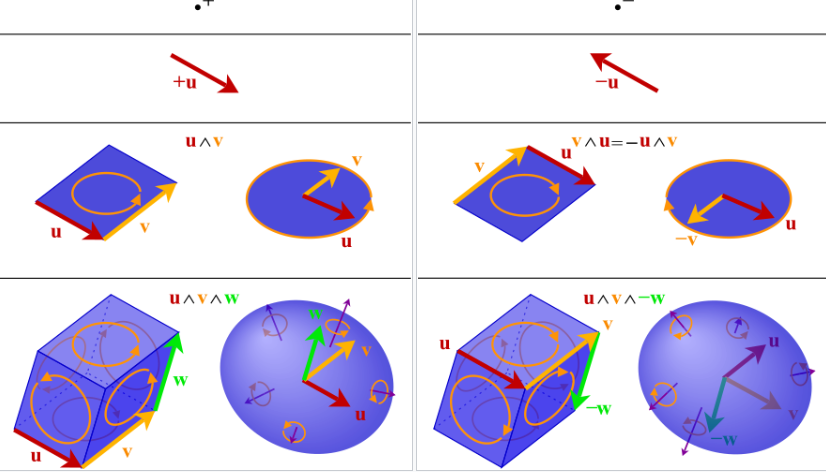
\includegraphics[scale =0.8]{wedge}
		\caption{Oriented $k$-volume of parallelopiped spanned by an ordered set of $k$-vectors. Changing the order corresponds to changing the orientation.}
	\end{center}
\end{figure}


\begin{theorem}[Universal property of exterior products]
	Let $V$ and $U$ be finite dimensional real vector spaces and denote by $\iota : V^k \to \bigwedge^k V$ the $k$-linear map $(v_1, \dots, v_k) \mapsto v_1 \wedge \dots \wedge v_k$. Then for every alternating $k$-linear map $\phi :V^k \to U$, there exists a unique linear map $\widetilde \phi : \bigwedge^k V \to U$ such that the diagram commutes
	\begin{center}
		\begin{tikzcd}
V^k \arrow[r, "\iota"] \arrow[rd, "\phi"'] & \bigwedge^k V \arrow[d, "\widetilde \phi"] \\
                                           & U                                         
\end{tikzcd}
	\end{center}
\end{theorem}

\begin{proof}
	By the universal property for tensor products, the $k$-linear map $\phi : V^k \to U$ descends uniquely to a linear map $\overline \phi : V^{\otimes k} \to U$ satisfying 
		\[ \overline \phi (v_1 \otimes \dots \otimes v_k) = \phi(v_1, \dots, v_k). \]
	We see from the alternating property of $\phi$ that $I \hookrightarrow  \ker \overline \phi$, so $\overline \phi$ descends to $\widetilde \phi : \bigwedge^k V \to U$ the unique linear map satisfying 
		\[ \widetilde \phi (v_1 \wedge \dots \wedge v_k) = \overline (v_1 \otimes \dots \otimes v_k) = \phi(v_1, \dots, v_k). \]
	The condition above can be rewritten as $\widetilde \phi \circ \iota = \phi$, completing the proof. 		
\end{proof}

\begin{corollary}
	If $V$ is a vector space of dimension $n$ and $\{e_1, \dots, e_n\}$ is a basis for $V$, then 
	\[ \{ e_{i_1} \wedge \dots \wedge e_{i_k} : i_1 < \dots, i_k \} \]
forms a basis for $\bigwedge^k V$, which therefore has dimension $\binom{n}{k}$ when $k \leq n$ and dimension zero when $k > n$.
\end{corollary}

\subsection{Orientation}

Let $V$ be a real vector space of dimension $n$, denote $\Fr (V)$ the space of ordered bases of $V$, known as \emph{frames}. Choosing a frame $(v_1, \dots, v_n) \in \Fr (V)$ induces a bijection $\GL_n (V) \to \Fr (V)$ by 
	\[ A \mapsto (Av_1, \dots, Av_n). \]
This bijection induces a smooth structure on the space of frames such that $\GL_n (V) \cong \Fr (V)$. Under the induced topology, there are two connected components of $\Fr(V)$ which we call \emph{orientations} of $V$. 

\subsection{Pullbacks and pushforwards}

Let $A: V \to W$ be a linear map between vector spaces. 


\section{Vector bundles}

Let $M$ be a manifold, and suppose $\{ E_p \}_{p \in M}$ is a family of real vector spaces of dimension $k$. Set
	\[ E := \bigsqcup_{p \in M} E_p \]
and define the projection $\pi : E \to M$ by its fibres $\pi^{-1} (p) = E_p$. We say that $(E, \pi)$ is a \emph{vector bundle of rank $k$} if $E$ is a manifold and $\pi$ is a smooth map admitting \emph{local trivialisations}, i.e. for every $p \in M$ there exists an open neighborhood $U \subseteq M$ and a diffeomorphism $\pi^{-1} (U) \xrightarrow{\sim} U \times \R^k$ which restricts to a vector space isomorphism $\pi^{-1} (p) \xrightarrow{\sim} \R^k$. 

\begin{figure}[h]
	\begin{center}
		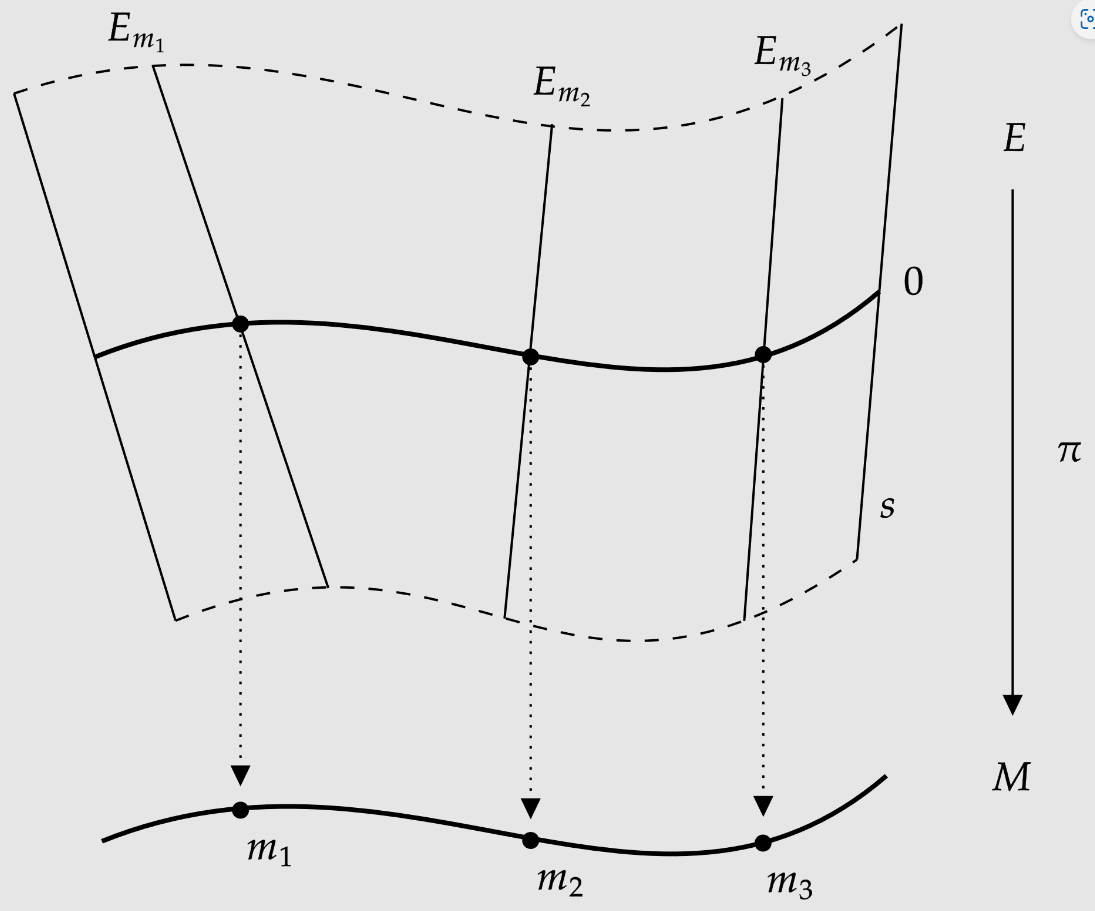
\includegraphics[scale = 0.3]{bundle}
		\caption{We can think of a vector bundle $E$ as a smooth ``attachment'' of a family of vector spaces $\{E_p\}_{p \in M}$ to the base manifold $M$.}
	\end{center}	
\end{figure}

A \emph{section} of a vector bundle $\pi : E \to M$ is a smooth map $\sigma : M \to E$ such that $\pi \circ \sigma : M \to M$ is the identity. 
Noting that $\sigma(p) \in E_p$ for each $p \in M$, the space of sections, denoted by $\Gamma (E)$, forms a real vector space under pointwise addition and scalar multiplication, 
	\[ (\sigma_1 + \lambda \sigma_2) (p) := \sigma_1 (p) + \lambda \sigma_2 (p), \]
and a $C^\infty (M)$-module under pointwise multiplication, 
	\[  (f\sigma)(p) := f(p) \sigma(p). \]
	
	\begin{figure}[h]
	\begin{center}
		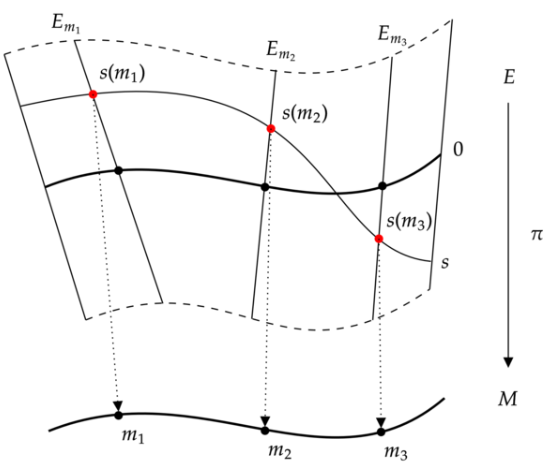
\includegraphics[scale = 0.5]{section}
		\caption{We can think of a section $\sigma : M \to E$ as a smooth ``attachment'' of a family of vectors $\{\sigma (p)\}_{p \in M}$ to the base manifold $M$.}
	\end{center}	
\end{figure}

\begin{example}
	Let $M$ be a manifold of dimension $n$, the \emph{tangent bundle} $\pi : TM \to M$ is defined as
		\[ TM := \bigsqcup_{p \in M} T_p M. \]
	To topologise $TM$, let $U \subseteq M$ be an open set with coordinates $x$, since an element $v \in T_p M$ can be written as $\sum_i a_i \tfrac{\partial}{\partial x_i}$, we identify $\pi^{-1} (U) \xrightarrow{\sim} U \times \R^n$ via the bijection
		\[ (p, v) \mapsto (x, a). \]
	Given $(x, a)$ coordinates on $	U \times \R^n$ and $(y, b)$ coordinates on $V \times \R^n$, we compute the transition map,
		\[ \sum_i a_i \frac{\partial}{\partial x_i} = \sum_{i, j} a_i \frac{\partial y_j}{\partial x_i} \frac{\partial}{\partial y_j} \]	
	hence $(x, a) \mapsto (y, \frac{\partial y}{\partial x} a)$. Thus the transition maps are smooth and $TM$ admits a smooth structure. Sections of the tangent bundle $\sigma : M \to TM$ are known as \emph{vector fields}, and the space of sections is denoted $\mathfrak X(M) := \Gamma (TM)$. 
\end{example}

\subsection{Construction}

Let $\Phi_\alpha : \pi^{-1} (U_\alpha) \xrightarrow{\sim} U_\alpha \times \R^k$ be local trivialisations of the vector bundle $\pi : E \to M$, then the transition functions $\Phi_\beta \circ \Phi^{-1}_\alpha : (U_\alpha \cap U_\beta) \times \R^k \to (U_\alpha \cap U_\beta) \times \R^k$ take the form 
	\[ \Phi_\alpha \circ \Phi^{-1}_\beta : (p, v) \mapsto (p, \tau_{\beta\alpha} (p) v) \]
for smooth $\tau_{\alpha \beta} : U_\alpha \cap U_\beta \to \GL(\R^k)$ satisfying the \emph{cocycle conditions}
	\begin{alignat*}{2}
		\tau_{\alpha \alpha}
			&= I, && \qquad \text{on $U_\alpha$}\\
		\tau_{\alpha \beta} \tau_{\beta \alpha}
			&= I, && \qquad \text{on $U_\alpha \cap U_\beta$}\\
		\tau_{\beta \gamma} \tau_{\alpha \beta} 
			&= \tau_{\alpha \gamma} && \qquad \text{on $U_\alpha \cap U_\beta \cap U_\gamma$}.
	\end{alignat*}
In fact, the cocycle conditions completely characterise a vector bundle in that given a family $\{ \tau_{\alpha \beta} \}_{\alpha, \beta}$ of smooth functions satisfying the cocycle conditions, there exists a unique vector bundle whose transition functions are given by $\tau_{\alpha \beta}$. 

\begin{remark}
	For the tangent bundle $TM$, the transition functions were given by the Jacobian matrices $\tau_{\alpha \beta} = \tfrac{\partial y}{\partial x}$ for coordinates $x$ on $U_\alpha$ and $y$ on $U_\beta$. For coordinates $z$ on $U_\gamma$, the cocycle condition is in fact the chain rule,
		\[ \frac{\partial z}{\partial y} \frac{\partial y}{\partial x} = \frac{\partial z}{\partial x}.\]
\end{remark}

\begin{theorem}[Vector bundle construction]
	Let $M$ be a manifold, $\{U_\alpha\}_\alpha$ an open cover, and $\tau_{\alpha \beta} : U_\alpha \cap U_\beta \to \GL (\R^k)$ smooth maps satisfying the cocycle conditions. Then there exists a unique vector bundle $E \to M$ of rank $k$ with local trivialisations $\pi^{-1} (U_\alpha) \xrightarrow{\sim} U_\alpha \times \R^k$ whose transition functions are given by $\tau_{\alpha \beta}$.
\end{theorem}

\begin{proof}
	Define
		\[ E :=\left( \bigsqcup_{\alpha} U_\alpha \times \R^k \right) / \sim,  \]
	where the relation $(\alpha, p, v) \sim (\beta, q, w)$ holds if and only if $p = q$ and $\tau_{\alpha \beta} (p) v = w$. We claim that this is an equivalence relation; let $(\alpha, p, v) \sim (\beta, q, w)$ and $(\beta, q, w) \sim (\gamma, r, u)$, then the relation satisfies
	\begin{itemize}
		\item reflexivity, $(\alpha, p, v) \sim (\alpha, p, v)$ by the first cocycle condition, 
		
		\item symmetry, $(\beta, q, w) \sim (\alpha, p, v)$ by the second cocycle condition, 
		
		\item transitivity, $(\alpha, p, v) \sim (\gamma, r, u)$ by the third cocycle condition. 
	\end{itemize}
	It is easy to see that the projection map $\pi : E \to M$ given by $\pi(\alpha, p, v) := p$ is well-defined with respect to the equivalence relation and that the fibres $E_p := \pi^{-1} (p)$ form $k$-dimensional vector spaces. We endow $E$ with a smooth structure via the maps $\Phi_\alpha : \pi^{-1} (U_\alpha) \to U_\alpha \times \R^k$ defined by $\Phi_\alpha (\beta, p, w) := (p, \tau_{\beta \alpha} (p) v)$. This is a well-defined injection; indeed, 
		\[ \Phi_\alpha (\beta, p, v) = (p, \tau_{\beta \alpha}(p) v) = (q, \tau_{\gamma \alpha} (q) w) = \Phi_\alpha (\gamma, q, w) \]	
	if and only if $p = q$ and $\tau_{\beta \alpha} (p) v = \tau_{\gamma \alpha} (q) w$ if and only if, by the cocycle conditions, $(\beta, p, v) \sim (\gamma, q, w)$. It is clear that $\Phi_\alpha$ is surjective, so it topologises $E$. Furthermore, the transition maps are of the form
		\[ (\Phi_\alpha \circ \Phi_\beta^{-1})(p, v) = \Phi_\alpha (\beta, p, v) = (p, \tau_{\beta \alpha} (p) v) \]
	and hence smooth. This completes the proof. 
\end{proof}

The vector bundle construction theorem gives a convenient way not only of constructing vector bundles, but also building new bundles from old. For example, we can use a homomorphism $\rho : \GL (\R^k) \to \GL (V)$, known as a \emph{representation}, to \textit{twist} a vector bundle $\pi : E \to M$ of rank $k$.

\begin{corollary}[Twisted vector bundle]
	Let $\pi : E \to M$ be a vector bundle of rank $k$ with transition functions $\tau_{\alpha \beta}$, and suppose $V$ is a real vector space of dimension $n$. If $\rho : \GL (\R^k) \to \GL (V)$ is a representation, then there exists a unique rank $m$ vector bundle $E \times_\rho V$ with transition functions $\rho (\tau_{\alpha \beta})$. 
\end{corollary}

\begin{proof}
	It suffices to show $\rho \circ \tau_{\alpha \beta}$ satisfy the cocycle conditions. Indeed, 
	\begin{align*}
		\rho(\tau_{\alpha \alpha})
			&= \rho (I) = I, \\
		\rho (\tau_{\alpha \beta}) \rho ( \tau_{\beta \alpha})
			&= \rho (\tau_{\alpha \beta} \tau_{\beta \alpha}) = \rho (I) = I, \\
		\rho(\tau_{\beta \gamma}) \rho( \tau_{\alpha \beta}) 
			&=\rho(\tau_{\beta \gamma}\tau_{\alpha \beta})  = \rho( \tau_{\alpha \gamma}).
	\end{align*}
	By the vector bundle construction theorem, we are done. 
\end{proof}

\begin{example}
	The representation 
		\begin{align*}
			\GL (\R^n) 
				&\to \GL (\R)\\
			A
				&\mapsto \det A				
		\end{align*}
	twists the tangent bundle $TM$ to form the line bundle $\bigwedge^n TM$. The representation
		\begin{align*}
			\GL (\R^n) 
				&\to \GL (\R^n)\\
			A
				&\mapsto (A^{-1})^*			
		\end{align*}
	twists the tangent bundle $TM$ to form the cotangent bundle $T^* M$. 	
\end{example}

	

\subsection{Orientability}

The general linear group $\GL (\R^k)$ has two connected components, the subgroups $\GL^+ (\R^k)$ and $\GL^- (\R^k)$ with positive and negative determinants. We say that a vector bundle $\pi : E \to M$ is \emph{orientable} if there exists a subcover $\{U_\alpha\}_\alpha$ of $M$ and transition functions $\tau_{\alpha \beta} : U_\alpha \cap U_\beta \to \GL (\R^k)$ which factor through $\GL^+ (\R^k)$. 

We say manifold $M$ is \emph{orientable} if the tangent bundle is orientable. In more detail, $M$ is orientable if there exists a sub-atlas $\{\phi_\alpha : U_\alpha \to \R^n\}_\alpha$ such that the Jacobians $d(\phi_\beta \circ \phi_\alpha^{-1} : U_\alpha \cap U_\beta \to \GL (\R^n)$ have positive determinant. We refer to this atlas as an \emph{oriented atlas}. 

\begin{example}
\leavevmode
\begin{enumerate}
	\item The real projective space $\mathbb{RP}^2$ is the quotient of the sphere $S^2$ under identifying antipodal points $x \sim - x$. By following an oriented basis from $x$ to $-x$, we find that $\mathbb{RP}^2$ is not orientable. 
	
	\item The Mobius band is the quotient manifold of $[0, 1] \times \R$ under identifying $(0, t) \sim (1, -t)$. By following an oriented basis along the length of a band, we see that the orientation is reversed upon crossing $\{1\} \times \R$. 
	
	\item Every complex manifold is orientable, since $\GL (\C^n) \subseteq \GL^+ (\R^{2n})$. 
\end{enumerate}
\end{example}


\section{Differential forms}

Let $M$ be a manifold, the vector bundle of $k$-th exterior powers of the cotangent space is formed by twisting the cotangent bundle $T^*M$ with the representation $A \mapsto A \wedge \dots \wedge A$, thereby taking the form
	\[ \bigwedge^k T^* M := \bigsqcup_{p \in M} \bigwedge^k T^*_p M. \]
A \emph{differential $k$-form} is a section of this vector bundle, and we denote the space of differential $k$-forms by $\Omega^k (M) := \Gamma (\bigwedge^k T^*M)$, and by convention the space of $0$-forms is taken to be the smooth functions. Intuitively, a differential $k$-form assigns an ``oriented $k$-density'' to every point in $p \in M$. In local coordinates $x$, a $k$-form $\omega \in \Omega^k (M)$ takes the form
	\[ \omega = \sum_{i_1 < \dots < i_k} f_{i_1, \dots, i_k} (x) dx^{i_1} \wedge \dots \wedge dx^{i_k}\]
where the coefficient $f_{i_1, \dots, i_k}$ is smooth on the local coordinate chart. 

\subsection{Exterior derivative and pullback}

Let $\phi : M \to N$ be a smooth map, then, choosing local coordinates $x$ and $y$ on $M$ and $N$ respectively, the \emph{pullback} $\phi^* : \Omega^k (N) \to \Omega^k (M)$ is
		\[ \phi^* \omega := \sum_{i_1 < \dots < i_k} (f_{i_1, \dots, i_k} \circ \phi) \wedge d(x^{i_1} \circ \phi) \wedge \dots \wedge d(x^{i_k} \circ \phi).\]
The \emph{exterior derivative} $d : \Omega^{k} (M) \to \Omega^{k + 1} (M)$ is the unique extension of the differential on smooth functions to a graded derivation on the algebra of differential forms, that is, 
\begin{enumerate}
	\item if $f \in \Omega^0 (M)$, then $df \in \Omega^1 (M)$ is the differential, 
	
	\item $d$ is linear, and if $\alpha \in \Omega^k (M)$ and $\beta \in \Omega^l (M)$, then $d$ satisfies the anti-commutative product rule
		\[ d(\alpha \wedge \beta) = (d \alpha) \wedge \beta + (-1)^k \alpha \wedge (d \beta), \]
	
	\item $d$ is nilpotent, $d^2 = 0$. 
\end{enumerate}
In local coordinates $x$, the exterior derivative of a $0$-form $f \in \Omega^0 (M)$ and a $k$-form $\omega \in \Omega^k (M)$ take the form
	\begin{align*}
		df
			&= \sum_{i} \frac{\partial f}{\partial x^i} dx^i, \\
		d \omega
			&= \sum_{i_1 < \dots < i_k} df_{i_1, \dots, i_k} \wedge dx^{i_1} \wedge \dots \wedge dx^{i_k}.
	\end{align*}
Upon checking coordinate invariance, one can take this coordinate representation as the definition of the exterior derivative and check that it satisfies the desired properties, hence establishing existence. Furthermore, localising we see that any exterior derivative must take the form above in local coordinates, establishing uniqueness. 

\begin{proposition}
	The exterior derivative commutes with the pullback. 
\end{proposition}

\begin{proof}
	We first prove the result for $0$-forms. Let $f \in \Omega^0 (N)$ and $p \in M$, then 
		\[ d  \phi^*f(p) = d(f \circ \phi) (p) = [f \circ \phi - f \circ \phi(p)] = \phi^* df (p). \]
	For an arbitrary $k$-form, we have
	\begin{align*}
		d \phi^* \omega
			&= d \sum_I \phi^* f d(x^I \circ \phi) = \sum_I d\phi^* f \, d(x^I \circ \phi), \\
		\phi^* d \omega
			&= \phi^* \sum_I df \wedge d x^I = \sum_I \phi^* d f \wedge d (x^I \circ \phi) = \sum_I d\phi^* f \wedge d(x^I \circ \phi).	
	\end{align*}
\end{proof}

\subsection{Orientation}

Earlier we defined the \textit{property} of orientability, we now make precise the notion of an orientation. We will need the following equivalent characterisation of orientability of a manifold;

\begin{proposition}
	An $n$-dimensional manifold $M$ is orientable if and only if there exists a nowhere vanishing $n$-form. 
\end{proposition}

\begin{proof}
	Suppose $M$ is orientable, and let $\{ \phi_\alpha: U_\alpha \to \R^n \}_\alpha$ be an oriented atlas, i.e. the transition functions $\tau_{\alpha \beta} := d(\phi_\alpha \circ \phi_\beta^{-1})$ have positive determinant. Take a partition of unity $\{f_\alpha\}_\alpha$ subordinate to the cover $\{U_\alpha \}_\alpha$, and choose $x^1_\alpha, \dots, x^n_\alpha$ coordinates on $U_\alpha$. Set
		\[ \omega := \sum_\alpha f_\alpha dx^1_\alpha \wedge \dots dx^n_\alpha, \]
	we claim that $\omega$ is nowhere vanishing. Indeed, changing variables, 
		\[ (\phi_\beta \circ \phi_\alpha^{-1})^* \omega = \sum_\alpha f_\alpha \circ (\phi_\alpha \circ \phi_\beta^{-1}) \det (\tau_{\alpha \beta}) \, dx^1_\beta \wedge \dots \wedge dx^n_\beta. \]	
	At any point $p \in M$, there exists $\alpha$ such that $f_\alpha (p) > 0$, while the other terms contribribute non-negatively since $f_\alpha \circ (\phi_\alpha \circ \phi_\beta^{-1}) \det (\tau_{\alpha \beta})  \geq 0$. This proves the claim. 
		
	Conversely, suppose there exists a non-vanishing $n$-form $\omega \in \Omega^n (M)$, then we choose a sub-atlas whose coordinate functions $x^1_\alpha, \dots, x^n_\alpha$ satisfy the condition that in these coordinates
		\[ \omega = f dx^1_\alpha \wedge \dots \wedge dx^n_\alpha\]
	for $f > 0$. It is clear then that the transition functions have positive determinant. 	
\end{proof}

\begin{remark}
	The existence of a non-vanishing $n$-form induces a vector bundle isomorphism $\bigwedge^n T^* M \cong M \times \R$, i.e. $\bigwedge^n T^* M$ is a trivial vector bundle. 
\end{remark}

On a connected manifold $M$, any two non-vanishing $n$-forms $\omega$ and $\eta$ differ by either a positive or negative function $f \in C^\infty (M)$ such that $\omega = f \eta$. Defining the equivalence relation $\omega \sim \eta$ via $\omega = f \eta$ for $f$ positive, then $\Omega^n (M)$ factors into two equivalence classes known as \emph{orientations} of $M$. 

\subsection{Integration}

Let $M$ be a manifold with oriented atlas $\{\phi_\alpha : U_\alpha \to \R^n\}_\alpha$, and choose a partition of unity $\{f_\alpha\}_\alpha$ subordinate to the cover $\{U_\alpha\}_\alpha$. Then the \emph{integral} of a differential $n$-form $\omega \in \Omega^n (M)$ is defined as
	\[ \int_M \omega := \sum_\alpha \int_{U_\alpha} (\phi^{-1}_\alpha)^* (\rho_\alpha \omega). \]
To illustrate the importance of orientability, we will verify that this definition is independent of choice of atlas and partition of unity. Let $\{ \psi_\beta : V_\beta \to \R^n \}$ be an oriented atlas and $\{g_\beta\}$ be a partition of unity subordinate to $\{V_\beta\}$. Fix $\alpha$ and $\beta$ such that $U_\alpha \cap V_\beta \neq \varnothing$ and write $\phi_\alpha = (x_1, \dots, x_n)$ and $\psi_\beta = (y_1, \dots, y_n)$. Then in coordinates
		\[ \omega = f dx_1 \wedge \dots \wedge dx_n = (f \circ \phi_\alpha \circ \psi_\beta^{-1})\det D(\phi_\alpha \circ \psi_\beta^{-1}) dy_1 \wedge \dots \wedge dy_n.  \]
	 Our goal is to verify
		\[ \int_{\phi_\alpha (U_\alpha)} \left( \phi_\alpha^{-1} \right)^* (f_\alpha g_\beta \omega) = \int_{\psi_\beta (V_\beta)} \left( \psi_\alpha^{-1} \right)^* (f_\alpha g_\beta \omega)\]
	Note $\phi_\alpha \circ \psi^{-1}_\beta$ is a diffeomorphism with $\det D(\phi_\alpha \circ \psi_\beta^{-1}) > 0$ and $f_\alpha g_\beta \omega$ is supported on $U_\alpha \cap V_\beta$, so the integrals can be equivalently taken over $\phi_\alpha (U_\alpha \cap V_\beta)$ and $\psi_\beta (U_\alpha \cap V_\beta)$ respectively. The result holds on $\R^n$; indeed by the change of variables formula, writing $G = x \circ y^{-1}$ for the positive orientation change of variables, 
		\begin{align*}
			\int_{\R^n} \omega = \int_{\R^n} f dx^1 \wedge \dots dx^n = \int_{\R^n} (f \circ G) \left| \det dG \right| dy^1 \wedge \dots \wedge dy^n = \int_{\R^n} G^* \omega.
		\end{align*}
	We extend this result to forms on $M$, since $\sum_\alpha f_\alpha = \sum_\beta g_\beta = 1$ we obtain
		\begin{align*}
			\sum_\alpha \int_{\phi_\alpha (U_\alpha)} \left( \phi_\alpha^{-1} \right)^* (f_\alpha \omega)
				&= \sum_\alpha \sum_\beta \int_{\phi_\alpha (U_\alpha)} \left( \phi_\alpha^{-1} \right)^* (f_\alpha g_\beta \omega) \\
				&= \sum_\alpha \sum_\beta  \int_{\psi_\beta (V_\beta)} \left( \psi_\beta^{-1} \right)^* (f_\alpha g_\beta \omega) = \sum_\beta \int_{\psi_\beta (V_\beta)} \left( \psi_\beta^{-1} \right)^* (g_\beta \omega). 
		\end{align*}

\begin{theorem}[Stokes' theorem]
	Let $M$ be an oriented manifold of dimension $n$ with boundary, and suppose $\omega \in \Omega^{n - 1} (M)$ is compactly supported. Then 	
		\[ \int_M d \omega = \int_{\partial \Omega} \omega. \]
\end{theorem}

\begin{proof}
	Choose an open cover $\{U_\alpha \}_\alpha$ of $M$ such that either 
		\[ U_\alpha \cong (0, 0)^n, \qquad \text{or} \qquad U_\alpha \cong (0, 1)^{n - 1} \times (0, 1]. \]
	Let $\{\rho_\alpha\}_\alpha$ be a partition of unity subordinate to the cover, then by linearity it suffices to show that 
		\[ \int_{U_\alpha} d(\rho_\alpha \omega) = \int_{\partial M \cap U_\alpha} \rho_\alpha \omega. \]
	We prove the $n = 2$ case, the general case follows similarly. In local coordinates, a compactly supported form $\omega \in \Omega^1 ((0, 1] \times [0, 1])$ takes the form $\omega = f_1 dx^1 + f_2 dx^2$, then by compact support, 
		\begin{align*}
			\int_{\partial M} \omega 
				&= \int_{\partial M} f_1 dx^1 + f_2 dx^2 = \int_0^1 f_2 (1, x^2) dx^2
		\end{align*}
	and by the fundamental theorem of calculus	
		\begin{align*}		
			\int_M d \omega
				&= \int_0^1 \int_0^1 \left( - \frac{\partial f_1}{\partial x^2} + \frac{\partial f_2}{\partial x^1} \right) dx^1 dx^2	\\
				&= \int_0^1 \left( \frac{\partial f_2}{\partial x^1} dx^1 \right) dx^2 + \int_0^1 \left( - \frac{\partial f_1}{\partial x^2} dx^2 \right) dx^1 \\
				&= \int_0^1 f_2 (1, x^2) - f_2 (0, x^2)) \, dx^2 + \int_0^1 (f_1 (x^1, 0) - f_1 (x^1, 1)) \, dx^1 = \int_0^1 f_2 (1, x^2) \, dx^2. 
		\end{align*}		
	This completes the proof. 	
\end{proof}

\begin{corollary}[Integrals of exact forms]
	Let $M$ be a compact oriented manifold without boundary, then the integral of every exact $n$-form $d \omega \in \Omega^n (M)$ over $M$ is zero, 
		\[ \int_M d \omega = 0. \]
\end{corollary}

\begin{corollary}[Integrals of closed forms]
	Let $M$ be a compact oriented manifold with boundary, then the integral of every closed $(n - 1)$-form $\omega \in \Omega^{n - 1} (M)$ over $\partial M$ is zero, 
		\[ \int_{\partial M} \omega = 0. \]
\end{corollary}

\section{de Rham cohomology}

The \emph{de Rham complex} of a manifold $M$ of dimension $n$ is a cochain complex of differential forms
	\[ 0 \longrightarrow \Omega^0 (M) \overset{d}{\longrightarrow}  \Omega^1 (M) \overset{d}{\longrightarrow} \dots \Omega^0 (M) \overset{d}{\longrightarrow} \Omega^n (M) \longrightarrow 0. \]
We say that a differential form $\omega \in \Omega^k (M)$ is \emph{closed} if $d\omega = 0$, and \emph{exact} if there exists $\eta \in \Omega^{k - 1} (M)$ such that $\omega = d \eta$. The property $d^2$ implies that every exact form is closed, and so we can form the \emph{$k$-th de Rham cohomology} of $M$ as the quotient space
	\[ H^k_{\text{dR}} (M) := \frac{\ker d : \Omega^k (M) \to \Omega^{k - 1} (M)}{\im d : \Omega^{k - 1} (M) \to \Omega^k (M)}. \]
The de Rham cohomology ``measures'' the degree to which the de Rham complex fails to be an exact sequence. If the $k$-th de Rham cohomology is trivial, $H^k_{\text{dR}} (M) = 0$, then every closed $k$-form is exact. 

\begin{example}
\leavevmode
\begin{enumerate}
	\item Let $M$ be a single point, then $\Omega^0 (M) = \R$ and $\Omega^k (M) = 0$ for all $k \geq 1$. Hence $H^0_{\text{dR}} (M) = \R$ and $H^k_{\text{dR}} (M) = 0$ for all $k \geq 1$. 
	
	\item The de Rham cohomology on $\R$ is trivial. Indeed, $\Omega^0 (\R) = C^\infty (\R)$ and $\Omega^1 (\R) = C^\infty (\R)$. In coordinates, the exterior derivative $d: \Omega^0 (\R) \to \Omega^1 (\R)$ takes the form
		\[ df = \frac{df}{dx} dx. \]
	The kernel is the space of constant functions, hence $H^0 (\R) = \R$. By the fundamental theorem of calculus, every $1$-form is exact, so $H^1 (\R) = 0$. 	
	
	\item In general $H^0 (M) \cong \R$ whenever $M$ is connected, since $df = 0$ if and only if $f$ is locally constant. 
	
	\item Viewing the circle as $S^1 \cong \R/\Z$, both $\Omega^0 (S^1)$ and $\Omega^1 (S^1)$ are the space of periodic functions on $\R$. By the fundamental theorem of calculus, $f dx \in \Omega^1 (S^1)$ is exact if and only if $\int_{S^1} f \, dx = 0$. Hence $H^1 (S^1) = \R$ and we have the exact sequence 
		\[ 0 \longrightarrow \R \longrightarrow \Omega^0 (S^1) \overset{d}{\longrightarrow} \Omega^1 (S^1) \overset{\int}{\longrightarrow} \R \longrightarrow 0. \]
\end{enumerate}
\end{example}

\subsection{Mayer-Vietoris sequences}

We can decompose a manifold and compute its cohomology from components with simpler cohomology via the \emph{Mayer-Vietoris sequence}. 

\begin{theorem}[Mayer-Vietoris sequence]
	Let $U, V \subseteq M$ be open such that $M = U \cup V$. Denote $\iota_U : U \to M$ and $\iota_V : V \to M$ and $\iota : U \sqcup V \to M$ the natural inclusion maps, 
		\[ U \cap V \overset{(\iota_U, \iota_V)}{\longrightarrow} U \sqcup V \overset{\iota}{\longrightarrow} M. \]
	Then we have the following long exact sequence:
	\begin{center}
\begin{tikzcd}
0 \arrow[r] & H^0 (M) \arrow[r, "\iota^*"] & H^0 (U) \oplus H^0 (V) \arrow[r, "\iota^*_U - \iota^*_V"] & H^0 (U\cap V) \arrow[lldd] \\
            &                              &                                                           &                            \\
            & H^1 (M) \arrow[r, "\iota^*"] & H^1 (U) \oplus H^1 (V) \arrow[r, "\iota^*_U - \iota^*_V"] & H^1 (U\cap V) \arrow[lldd] \\
            &                              &                                                           &                            \\
            & H^2 (M) \arrow[r]            & \dots                                                     &                           
\end{tikzcd}
	\end{center}
\end{theorem}

\subsection{Homotopy theory}

We say the two maps $\phi_0, \phi_1 : M \to N$ are \emph{homotopic} if there exists a smooth map $\Phi : M \times [0, 1] \to N$ forming a \emph{homotopy} $\phi_t (p) := \Phi(p, t)$ from $\phi_0$ to $\phi_1$. A map $\phi : M \to N$ is a \emph{homotopy equivalence} if there exists $\psi : N \to M$ such that $\phi \circ \psi : N \to N$ and $\psi \circ \phi : M \to M$ are homotopic to the identity maps on $N$ and $M$ respectively. 

\begin{lemma}
	Let $\phi_t : M \to M$ be a family of diffeomorphisms for $t \in [0, 1]$. Then for all $t \in [0, 1]$ the pullbacks $\phi^*_t$ induce the same map $H^k (M) \to H^k (M)$. 
\end{lemma}

\begin{proof}
	Consider a closed $k$-form $\omega \in \Omega^k (M)$, then by Cartan's magic formula
		\[ \frac{d}{dt} \phi^*_t \omega_{|t = t_0} = \phi^*_{t_0} (d \iota_{X_{t_0}} + \iota_{X_{t_0}} d) \omega = d (\phi^*_{t_0} \iota_{X_{t_0}} \omega). \]
	Hence $\omega$ is exact, and the difference
		\[ \phi^*_t \omega - \omega = \int_0^t \frac{d}{dt} \phi^*_t \omega_{|t = s} \, ds \]
	is also exact. This proves the result. 		
\end{proof}


\begin{theorem}[Homotopy invariance]
\leavevmode
\begin{enumerate}
	\item If $\phi_t : M \to N$ is a homotopy from $\phi_0$ to $\phi_1$, then $\phi_t^* : H^k (N) \to H^k (M)$ is independent of $t$. 
	\item A homotopy equivalence $\phi : M \to N$ induces an isomorphism on the cohomology $\phi^* : H^k (N) \to H^k (M)$. 
\end{enumerate}
\end{theorem}

\begin{proof}
\leavevmode
\begin{enumerate}
	\item We extend the homotopy to a map $\Phi : M \times \R \to N$. 
	
	\item 
\end{enumerate}
\end{proof}

\begin{corollary}[Poincare lemma]
	For $k \geq 1$, the $k$-th de Rham cohomology of Euclidean space is trivial, $H^k (\R^n) = 0$.
\end{corollary}

\begin{proof}
	We will show that $\R^n$ is homotopy equivalent to a point $\R^0$. Consider maps $\phi : \R^n \to \R^0$ and $\psi : \R^0 \to \R^n$ given by 
		\[ \phi(x) = 0, \qquad \psi(0) = 0.  \]
	It is clear that $\phi \circ \psi : \R^0 \to \R^0$ is the identity, while $\psi \circ \phi : \R^n \to \R^n$, which takes the form $(\psi \circ \phi)(x) = 0$, is homotopic to the identity map via $F: \R^n \times [0, 1] \to \R^n$ given by
		\[ F(x, t) := tx. \]
	By homotopy equivalence, we are done. 	
\end{proof}

\subsection{Degree theory}



\end{document}